\subsection{評価射、余評価射の応用}\label{chap-5.4-application-of-eval-coeval}
  評価射、余評価射を用いれば、集合の圏における圏の定義に現れる操作と等しくなるような写像を構成することができる。ここでは恒等射を得る操作と対角写像の構成を示すが、射の合成を行う操作$\mor{\circ}{\arset{Set}{B}{C}\times \arset{Set}{A}{B}}{\arset{Set}{A}{C}}$を構成することもできる。
  \begin{prop}[余評価射による恒等射の定義]\label{prop-def-identity-arrow-by-coeval}
    $\mor{\arset{Set}{A}{\pi_A}\circ ce}{1}{\arset{Set}{A}{A}}$は射集合$\arset{Set}{A}{A}$における恒等射を表す元である。

    \begin{center}
			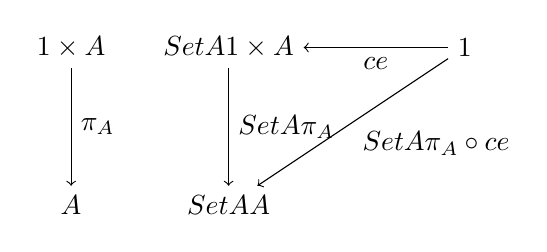
\begin{tikzpicture}[auto]
				\node (1a) at (0, 2) {$1\times A$};
        \node (a) at (0, 0) {$A$};
				\node (s1a) at (2, 2) {$\arset{Set}{A}{1\times A}$};
        \node (sa) at (2, 0) {$\arset{Set}{A}{A}$};
				\node (1) at (5, 2) {$1$};

				\draw[->] (1a) to node{$\pi_A$}(a);
        \draw[->] (s1a) to node{$\arset{Set}{A}{\pi_A}$}(sa);
        \draw[->] (1) to node{$ce$}(s1a);
        \draw[->] (1) to node{$\arset{Set}{A}{\pi_A}\circ ce$}(sa);

			\end{tikzpicture}
		\end{center}

  \end{prop}
  \begin{proof}
    $\arset{Set}{A}{\pi_A}\circ ce(*)$を計算すれば良い。\\
    \begin{align*}
      \arset{Set}{A}{\pi_A}\circ ce(*)&=\arset{Set}{A}{\pi_A}(\lambda x.\tuple{*,x})&\text{(写像の合成の定義)}\\
      &=\pi_A\circ\lambda x.\tuple{*,x}&\text{(射写像の定義)}\\
      &=\lambda x.\pi_A(\tuple{*,x})\\
      &=\lambda x.x\\
    \end{align*}
    余評価射の定義より任意の$A$の元$a$に対して$(\lambda x.x)(a)=a$であるから、$\arset{Set}{A}{\pi_A}\circ ce(*)=id_A$である。
  \end{proof}
  \begin{prop}[余評価射による対角写像の定義]\label{prop-def-diagonal-map-by-coeval}
    対角写像$\mor{\varDelta}{A}{\arset{Set}{B}{A}}$に対して、\[\varDelta=\arset{Set}{B}{\pi_A}\circ ce\]である。
    \begin{center}
			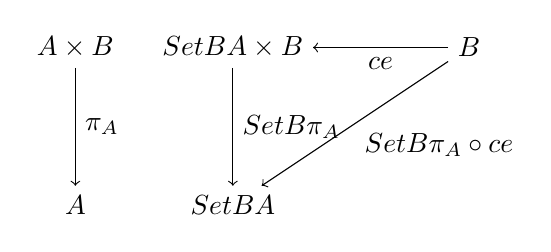
\begin{tikzpicture}[auto]
				\node (1a) at (0, 2) {$A\times B$};
        \node (a) at (0, 0) {$A$};
				\node (s1a) at (2, 2) {$\arset{Set}{B}{A\times B}$};
        \node (sa) at (2, 0) {$\arset{Set}{B}{A}$};
				\node (1) at (5, 2) {$B$};

				\draw[->] (1a) to node{$\pi_A$}(a);
        \draw[->] (s1a) to node{$\arset{Set}{B}{\pi_A}$}(sa);
        \draw[->] (1) to node{$ce$}(s1a);
        \draw[->] (1) to node{$\arset{Set}{B}{\pi_A}\circ ce$}(sa);
			\end{tikzpicture}
		\end{center}
  \end{prop}
  \begin{proof}
    $A$の任意の元$a$に対して、
    \begin{align*}
      \arset{Set}{B}{\pi_A}\circ ce(a)&=\arset{Set}{B}{\pi_A}(\lambda x.\tuple{a,x})&\text{(写像の合成の定義)}\\
      &=\pi_A\circ\lambda x.\tuple{a,x}&\text{(射写像の定義)}\\
      &=\lambda x.\pi_A(\tuple{a,x})\\
      &=\lambda x.a
    \end{align*}
    恒等射と同様に、$B$の任意の元$b$に対して$\mor{\lambda x.a}{B}{A}$は$(\lambda x.a)b=a$を満たす。よって$\lambda x.a$は定写像であり、$\lambda x.a=\varDelta (a)$である。\\
    $\arset{Set}{B}{\pi_A}\circ ce(a)=\varDelta (a)$が成り立つから、$\varDelta=\arset{Set}{B}{\pi_A}\circ ce$である。
  \end{proof}